\definecolor{myblue}{RGB}{56,94,141}
\newcommand\xsetpos{6}

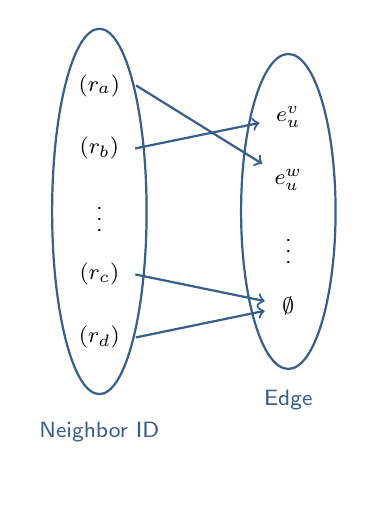
\begin{tikzpicture}[scale=.4,
                    arrow/.style={thick,->,myblue},
                    set name/.style={font=\color{myblue}\Large\bfseries\sf},
                    set/.style={thick,myblue},
                    every node/.style={circle},
                    font=\sf
                    ]
\draw[set] (0,0) circle [x radius=1.5cm, y radius=5.8cm]
           (\xsetpos,0) circle [x radius=1.5cm, y radius=5cm];

\node[set name] at (0,-7) {\footnotesize{Neighbor ID}};
\node[set name] at (\xsetpos,-6) {\footnotesize{Edge}};  

\node (a1) at (0,4)  {\footnotesize{$\id(r_a)$}};
\node (a2) at (0,2)  {\footnotesize{$\id(r_b)$}};
\node (a3) at (0,0) {\footnotesize{$\vdots$}};
\node (a4) at (0,-2) {\footnotesize{$\id(r_c)$}};
\node (a5) at (0,-4) {\footnotesize{$\id(r_d)$}};

\node (b1) at (\xsetpos,3)  {\footnotesize{$e_u^v$}};
\node (b2) at (\xsetpos,1)  {\footnotesize{$e_u^w$}};
\node (b3) at (\xsetpos,-1) {\footnotesize{$\vdots$}}; 
\node (b4) at (\xsetpos,-3) {\footnotesize{$\emptyset$}};
\begin{scope}[arrow]
  \draw (a1.east) -- (b2);
  \draw (a2.east) -- (b1);
  %\draw (a3.east) -- (b3);
  \draw (a4.east) -- (b4); 
  \draw (a5.east) -- (b4);
\end{scope}

\end{tikzpicture}    